\hypertarget{orshowsensors.cpp-example}{
\subsection{orshowsensors.cpp}
}
\begin{DoxyAuthor}{Author}
Rosen Diankov
\end{DoxyAuthor}
Shows how to toggle sensor power and rendering options

 
\begin{DoxyImage}
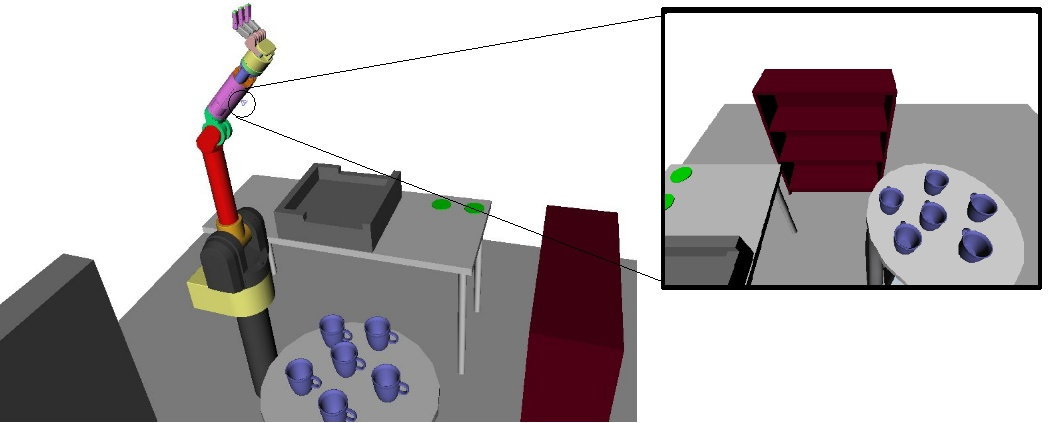
\includegraphics[width=20cm]{showsensors_camera.jpg}
\caption{Camera Sensor.}
\end{DoxyImage}


 
\begin{DoxyImage}
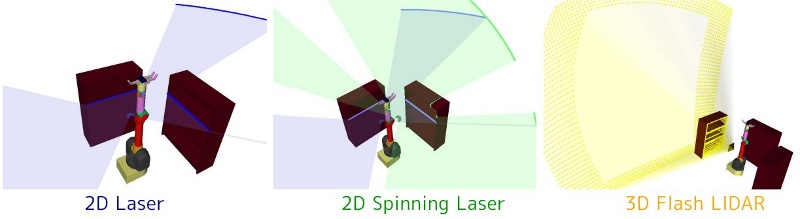
\includegraphics[width=20cm]{showsensors_laser.jpg}
\caption{Laser Sensor.}
\end{DoxyImage}


{\bfseries Full Example Code:}


\begin{DoxyCodeInclude}

#include <openrave-core.h>
#include <vector>

#include <boost/thread/thread.hpp>
#include <boost/bind.hpp>

#ifdef _WIN32
#define WIN32_LEAN_AND_MEAN
#include <winsock2.h>
#define usleep(micro) Sleep(micro/1000)
#endif

using namespace OpenRAVE;
using namespace std;

void SetViewer(EnvironmentBasePtr penv, const string& viewername)
{
    ViewerBasePtr viewer = RaveCreateViewer(penv,viewername);
    BOOST_ASSERT(!!viewer);

    // attach it to the environment:
    penv->AddViewer(viewer);

    // finally you call the viewer's infinite loop (this is why you need a separa
      te thread):
    bool showgui = true;
    viewer->main(showgui);
}

int main(int argc, char ** argv)
{
    RaveInitialize(true); // start openrave core
    EnvironmentBasePtr penv = RaveCreateEnvironment(); // create the main environ
      ment
    boost::thread thviewer(boost::bind(SetViewer,penv,"qtcoin"));
    penv->Load("data/testwamcamera.env.xml");
    size_t ienablesensor = 0;
    // get all the sensors, this includes all attached robot sensors
    std::vector<SensorBasePtr> sensors;
    penv->GetSensors(sensors);
    while(1) {
        for(size_t isensor = 0; isensor < sensors.size(); ++isensor) {
            sensors[isensor]->Configure(isensor == ienablesensor ? SensorBase::CC
      _PowerOn : SensorBase::CC_PowerOff);
            sensors[isensor]->Configure(isensor == ienablesensor ? SensorBase::CC
      _RenderDataOn : SensorBase::CC_RenderDataOff);
        }
        ienablesensor = (ienablesensor+1)%sensors.size();
        usleep(5000000); // 5s
    }
    return 0;
}
\end{DoxyCodeInclude}
 